\documentclass[a4paper, 12pt]{article}

\usepackage[top=2cm, bottom=2cm, left=2.5cm, right=2.5cm]{geometry}
\usepackage[utf8]{inputenc}
\usepackage{array}
\usepackage{verbatim}
\usepackage{graphicx}
\usepackage{hyperref}

\graphicspath{{img/}}

\begin{document}

\includegraphics{logo}\\
\textbf{UNIVERSIDADE ESTADUAL DE PONTA GROSSA} \\
SISTEMA UNIVERSIDADE ABERTA DO BRASIL - UAB \\
\underline{Licenciatura em Matemática | Polo UAB em Jacarezinho} \\
\textbf{ALUNO:} Ricardo Medeiros da Costa Junior   \textbf{RA:} 151774301 \\
\textbf{DISCIPLINA:} Instrumentação para o Ensino da Matemática IV \\
\textbf{ATIVIDADE:} Atividade 5 - Tarefa Descritiva (Valor: 5,0) \\

\begin{enumerate}
\item Analise os problemas matemáticos apresentados abaixo, tendo como referencial teórico o texto postado na unidade II: \textbf{“O ensino de matemática proposto nos PCN+ Ensino Médio e nas Diretrizes Curriculares da SEED/PR”}, quanto aos itens apresentados no quadro abaixo de cada questão.(Questões retiradas nas Olimpíadas de Matemática)
\begin{figure}[h!]
  \centering
  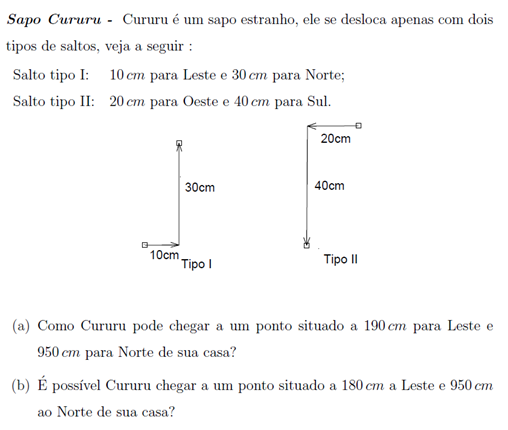
\includegraphics[width=0.5\textwidth]{1}
\end{figure} 
  \begin{enumerate}
  \item Eixo estruturante (PCN e DCE)\\\\
    Teste
  \item Conteúdo Matemático (Ensino Médio) \\\\
    Teste
  \item Conhecimentos matemáticos necessários para resolvê-la \\\\
    Teste
  \item Presença ou não da interdisciplinaridade \\\\
    Teste
  \item Presença de contextualização no texto da questão\\\\
    Teste
  \end{enumerate}
\newpage
\begin{figure}[h!]
  \centering
  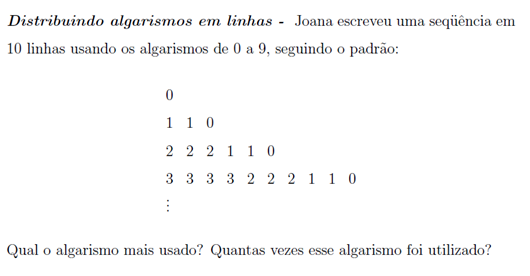
\includegraphics[width=0.5\textwidth]{2}
\end{figure} 
  \begin{enumerate}
  \item Eixo estruturante (PCN e DCE)\\\\
    Teste
  \item Conteúdo Matemático (Ensino Médio) \\\\
    Teste
  \item Conhecimentos matemáticos necessários para resolvê-la \\\\
    Teste
  \item Presença ou não da interdisciplinaridade \\\\
    Teste
  \item Presença de contextualização no texto da questão\\\\
    Teste
  \end{enumerate}
\begin{figure}[h!]
  \centering
  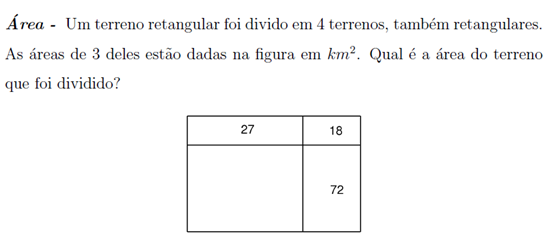
\includegraphics[width=0.5\textwidth]{3}
\end{figure} 
  \begin{enumerate}
  \item Eixo estruturante (PCN e DCE)\\\\
    Teste
  \item Conteúdo Matemático (Ensino Médio) \\\\
    Teste
  \item Conhecimentos matemáticos necessários para resolvê-la \\\\
    Teste
  \item Presença ou não da interdisciplinaridade \\\\
    Teste
  \item Presença de contextualização no texto da questão\\\\
    Teste
  \end{enumerate}
\end{enumerate}
\end{document}
